\documentclass[border=10pt]{standalone}
\usepackage{tikz}
\usetikzlibrary{arrows.meta}

% ========== 配色 ==========
\definecolor{inFill}{RGB}{183,224,177}
\definecolor{inLine}{RGB}{32,102,32}
\definecolor{hidFill}{RGB}{199,203,243}
\definecolor{hidLine}{RGB}{52,58,143}
\definecolor{outFill}{RGB}{243,199,199}
\definecolor{outLine}{RGB}{143,52,52}
\definecolor{orFill}{RGB}{250,224,180}
\definecolor{orLine}{RGB}{190,110,20}
\colorlet{myblue}{blue!70!black}

\begin{document}
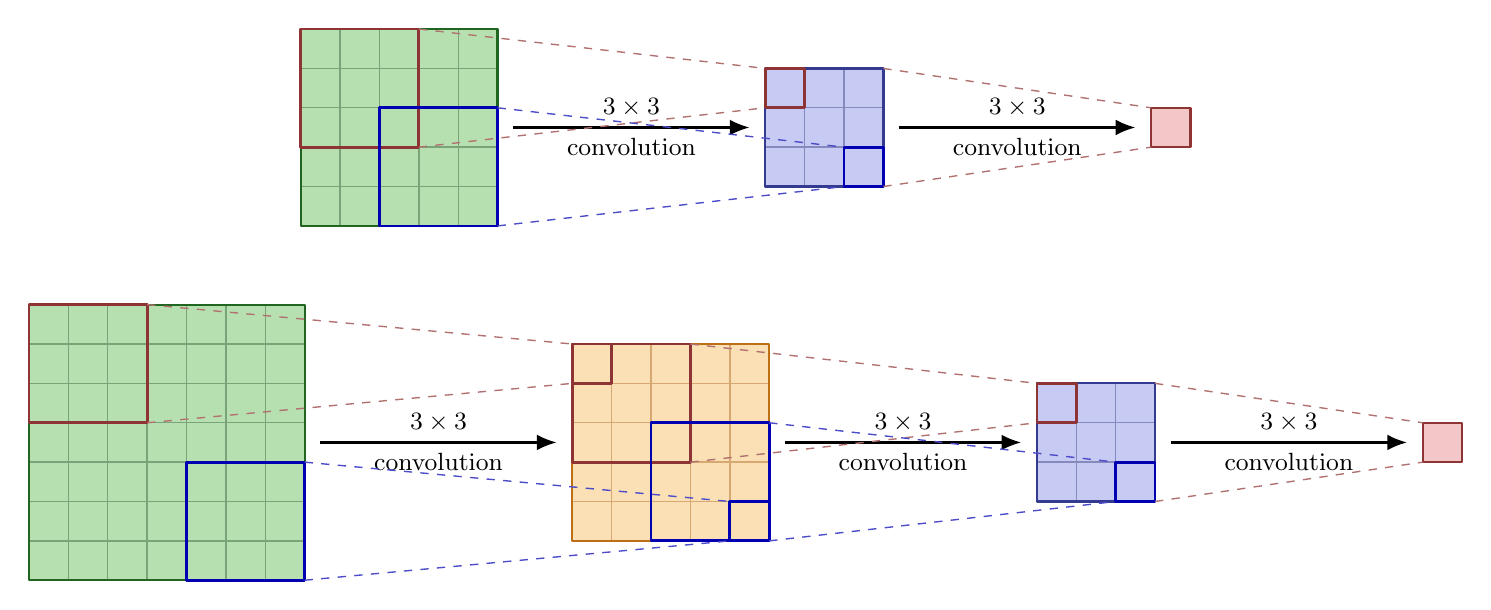
\begin{tikzpicture}[
    line join=round, font=\small, line width=.8pt,
    >={Latex[length=2.5mm, width=2mm]}
  ]

  % ========== 虚线宏：左框右两点 -> 右框左两点 ==========
  \newcommand{\conn}[8]{%
    \draw[#8, dashed, line width=.5pt]
      (#1+#3,#2+#4)--(#5,#6+#7)
      (#1+#3,#2)--(#5,#6);
  }

  % ================= 第一行：绿5x5 -> 紫3x3 -> 红1x1（不变）=================
  \begin{scope}[xshift=3.45cm]
    % ---- 输入 5x5（绿）----
    \fill[inFill] (0,0) rectangle (2.5,2.5);
    \draw[step=.5, inLine!60, line width=.5pt, shift={(0,0)}] (0,0) grid (2.5,2.5);
    \draw[inLine, thick] (0,0) rectangle (2.5,2.5);
    \draw[outLine, line width=1pt] (0,1) rectangle (1.5,2.5);
    \draw[myblue, line width=1pt] (1,0) rectangle (2.5,1.5);
    % ---- 第一层 3x3（紫）----
    \fill[hidFill] (5.9,0.5) rectangle (7.4,2.0);
    \draw[step=.5, hidLine!60, line width=.5pt, shift={(5.9,0.5)}] (0,0) grid (1.5,1.5);
    \draw[hidLine, thick] (5.9,0.5) rectangle (7.4,2.0);
    \draw[outLine, line width=1pt] (5.9,1.5) rectangle (6.4,2.0);
    \draw[myblue, line width=1pt] (6.9,0.5) rectangle (7.4,1.0);
    % ---- 第二层 1x1（红）----
    \fill[outFill] (10.8,1.0) rectangle (11.3,1.5);
    \draw[outLine, thick] (10.8,1.0) rectangle (11.3,1.5);
    % ---- 箭头 ----
    \draw[->] (2.7,1.25) -- node[above] {$3\times3$} node[below] {convolution} (5.7,1.25);
    \draw[->] (7.6,1.25) -- node[above] {$3\times3$} node[below] {convolution} (10.6,1.25);
    % ---- 虚线 ----
    \conn{0}{1}{1.5}{1.5}{5.9}{1.5}{.5}{outLine!70}
    \conn{1}{0}{1.5}{1.5}{6.9}{0.5}{.5}{myblue!70}
    \conn{5.9}{0.5}{1.5}{1.5}{10.8}{1.0}{.5}{outLine!70}
  \end{scope}

  % ================= 第二行：绿7x7 -> 橙5x5 -> 紫3x3 -> 红1x1 =================
  % ---- 输入 7x7（绿）----
  \fill[inFill] (0,-4.5) rectangle (3.5,-1.0);
  \draw[step=.5, inLine!60, line width=.5pt, shift={(0,-4.5)}] (0,0) grid (3.5,3.5);
  \draw[inLine, thick] (0,-4.5) rectangle (3.5,-1.0);
  \draw[outLine, line width=1pt] (0,-2.5) rectangle (1.5,-1.0);
  \draw[myblue, line width=1pt] (2,-4.5) rectangle (3.5,-3.0);
  % ---- 第一层 5x5（橙）----
  \fill[orFill] (6.9,-4.0) rectangle (9.4,-1.5);
  \draw[step=.5, orLine!60, line width=.5pt, shift={(6.9,-4.0)}] (0,0) grid (2.5,2.5);
  \draw[orLine, thick] (6.9,-4.0) rectangle (9.4,-1.5);
  \draw[outLine, line width=1pt] (6.9,-2.0) rectangle (7.4,-1.5);
  \draw[myblue, line width=1pt] (8.9,-4.0) rectangle (9.4,-3.5);
  % ★ 新增：紫层格子在橙层上的感受野 = 左上/右下 3x3 框
  \draw[outLine, line width=1pt] (6.9,-3.0) rectangle (8.4,-1.5);
  \draw[myblue, line width=1pt] (7.9,-4.0) rectangle (9.4,-2.5);
  % ---- 第二层 3x3（紫）----
  \fill[hidFill] (12.8,-3.5) rectangle (14.3,-2.0);
  \draw[step=.5, hidLine!60, line width=.5pt, shift={(12.8,-3.5)}] (0,0) grid (1.5,1.5);
  \draw[hidLine, thick] (12.8,-3.5) rectangle (14.3,-2.0);
  \draw[outLine, line width=1pt] (12.8,-2.5) rectangle (13.3,-2.0);
  \draw[myblue, line width=1pt] (13.8,-3.5) rectangle (14.3,-3.0);
  % ---- 第三层 1x1（红）----
  \fill[outFill] (17.7,-3.0) rectangle (18.2,-2.5);
  \draw[outLine, thick] (17.7,-3.0) rectangle (18.2,-2.5);
  % ---- 箭头 ----
  \draw[->] (3.7,-2.75) -- node[above] {$3\times3$} node[below] {convolution} (6.7,-2.75);
  \draw[->] (9.6,-2.75) -- node[above] {$3\times3$} node[below] {convolution} (12.6,-2.75);
  \draw[->] (14.5,-2.75) -- node[above] {$3\times3$} node[below] {convolution} (17.5,-2.75);
  % ---- 虚线 ----
  \conn{0}{-2.5}{1.5}{1.5}{6.9}{-2.0}{.5}{outLine!70}
  \conn{2}{-4.5}{1.5}{1.5}{8.9}{-4.0}{.5}{myblue!70}
  % ★ 修改：源框从 1x1 改为橙层上的 3x3 感受野框
  \conn{6.9}{-3.0}{1.5}{1.5}{12.8}{-2.5}{.5}{outLine!70}
  \conn{7.9}{-4.0}{1.5}{1.5}{13.8}{-3.5}{.5}{myblue!70}
  \conn{12.8}{-3.5}{1.5}{1.5}{17.7}{-3.0}{.5}{outLine!70}

\end{tikzpicture}
\end{document}